%% =====================================================================
%% NetPerturb -- Application Note for Bioinformatics Advances (OUP)
%%
%% FIRST DRAFT TEMPLATE. Everything marked \todo{...} (red) needs your input.
%%
%% Bioinformatics Advances limits for an Application Note (author guidelines):
%%   * up to 4 pages, including figures, tables and references
%%   * abstract: at most 200 words
%%   * at most 3 figures + tables COMBINED  (this draft: Fig 1, Fig 2, Table 1)
%%   * at most 15 references                 (this draft cites 15)
%%   * at most 5 keywords
%%   * required statements: Data availability, Funding, Conflict of interest,
%%     Author contributions; ORCID for the submitting author; any AI/LLM use
%%     must be disclosed in the cover letter and Methods/Acknowledgements
%%
%% Build:  latexmk -pdf netperturb.tex
%% =====================================================================

\documentclass[unnumsec,webpdf,contemporary,large]{oup-authoring-template}
%\onecolumn % for one column layouts

\graphicspath{{Fig/}}
\newcommand{\societylogo}{}

% Draft helpers -- remove before submission
\newcommand{\todo}[1]{\textcolor{red}{[TODO: #1]}}
\newcommand{\np}{\textsc{NetPerturb}}
\newcommand{\param}[1]{\texttt{-{}-#1}}

% line numbers (often requested by reviewers)
%\usepackage[right]{lineno}

\begin{document}

\journaltitle{Bioinformatics Advances}
\DOI{DOI added during production}
\copyrightyear{2026}
\pubyear{2026}
\vol{XX}
\issue{x}
\access{Published: Date added during production}
\appnotes{Application Note}

\firstpage{1}

\subtitle{Gene Regulation and Systems Biology} % \todo: confirm journal subject section

\title[NetPerturb]{NetPerturb: a reproducible Nextflow pipeline for in silico perturbation of single-cell gene regulatory networks from a Seurat object}

\author[1,$\ast$]{Diego Marques-Coelho\ORCID{0000-0000-0000-0000}}
\author[1]{\todo{Second Author}}
\author[2]{\todo{Third Author}}

\address[1]{\orgdiv{\todo{Department}}, \orgname{\todo{Organization}}, \orgaddress{\street{\todo{Street}}, \postcode{\todo{Postcode}}, \state{\todo{State}}, \country{\todo{Country}}}}
\address[2]{\orgdiv{\todo{Department}}, \orgname{\todo{Organization}}, \orgaddress{\street{\todo{Street}}, \postcode{\todo{Postcode}}, \state{\todo{State}}, \country{\todo{Country}}}}

\corresp[$\ast$]{Corresponding author. \href{mailto:diegomscoelho@gmail.com}{diegomscoelho@gmail.com}}

\received{Date}{0}{Year}
\revised{Date}{0}{Year}
\accepted{Date}{0}{Year}

\editor{Associate Editor: Name}

%% ---------------------------------------------------------------------
%% Abstract: <= 200 words, structured, no citations.
%% ---------------------------------------------------------------------
\abstract{
\textbf{Motivation:} Predicting how a genetic or pharmacological perturbation affects each cell population in a single-cell RNA-seq (scRNA-seq) dataset is a common question, but in silico perturbation tools based on gene regulatory networks (GRNs) are hard to install, scale poorly to large atlases, and return results that are difficult to compare across methods and to share.\\
\textbf{Results:} We present NetPerturb, a Nextflow pipeline that starts from a processed Seurat object and a list of target genes and returns a single, self-contained HTML report. NetPerturb balances cell identities by downsampling, checks the targets before any network is built, and infers one GRN per identity with GENIE3, scRank or hdWGCNA. It then ranks identities by a target-perturbation score. In parallel, it can run a virtual knockout with scTenifoldKnk, including joint knockouts of several genes, followed by gene set enrichment of the genes the knockout affects. Every stochastic step is seeded from one parameter and every tool runs in a versioned container, so runs are reproducible across HPC and cloud environments. On unstimulated PBMCs, interferon-stimulated genes scored highest in monocytes, a signal that remains after correcting for a cell-type-wide offset, and building the wild-type network once per identity cut the knockout cost about 24-fold.\\
\textbf{Availability and implementation:} NetPerturb is freely available under the \todo{MIT} licence at \url{https://github.com/MCBLab/NetPerturb}, with documentation, test profiles and container recipes. \todo{Zenodo DOI of the release.}\\
\textbf{Contact:} \href{mailto:diegomscoelho@gmail.com}{diegomscoelho@gmail.com}\\
\textbf{Supplementary information:} Supplementary data are available at \textit{Bioinformatics Advances} online.}

\keywords{single-cell RNA-seq, gene regulatory network, in silico perturbation, virtual knockout, Nextflow}

\maketitle

%% =====================================================================
\section{Introduction}
%% =====================================================================

Single-cell RNA-seq (scRNA-seq) resolves tissues into cell identities (cell types, clones, or treatment states), and the next question is usually which of those identities depend on a given gene or drug target. Pooled CRISPR screens with single-cell readout answer this experimentally \citep{Dixit2016perturbseq}, but they are costly and cannot be applied to archived or clinical samples. Computational alternatives therefore perturb a gene regulatory network (GRN) inferred from unperturbed cells and read the effect off the network: CellOracle simulates shifts in cell identity \citep{Kamimoto2023celloracle}, scRank ranks cell types by how much a drug target reshapes their network \citep{Li2024scrank}, and scTenifoldKnk performs a virtual knockout and reports the genes whose regulatory context changes \citep{Osorio2022sctenifoldknk}.

In practice, using these methods on a new dataset takes considerable engineering work. Each method expects its own input format and gene universe, and memory grows quickly with the number of cells and genes. Targets that are not expressed in some identities can end a run late in the analysis. Results from different network inference methods are rarely placed side by side, and many steps are stochastic, so the numbers are hard to reproduce. \todo{Add 1--2 sentences on the specific gap your lab hit.}

NetPerturb addresses this with a single Nextflow \citep{DiTommaso2017nextflow} workflow, organised following nf-core practice \citep{Ewels2020nfcore}. Its input is the object most analysts already have, a processed Seurat object \citep{Hao2023seurat}. It parallelises network inference and scoring across identities and targets, and it gathers every result, together with the quality control and provenance needed to interpret it, into one portable report.

%% =====================================================================
\section{Implementation}
%% =====================================================================

\begin{figure*}[!t]%
\centering
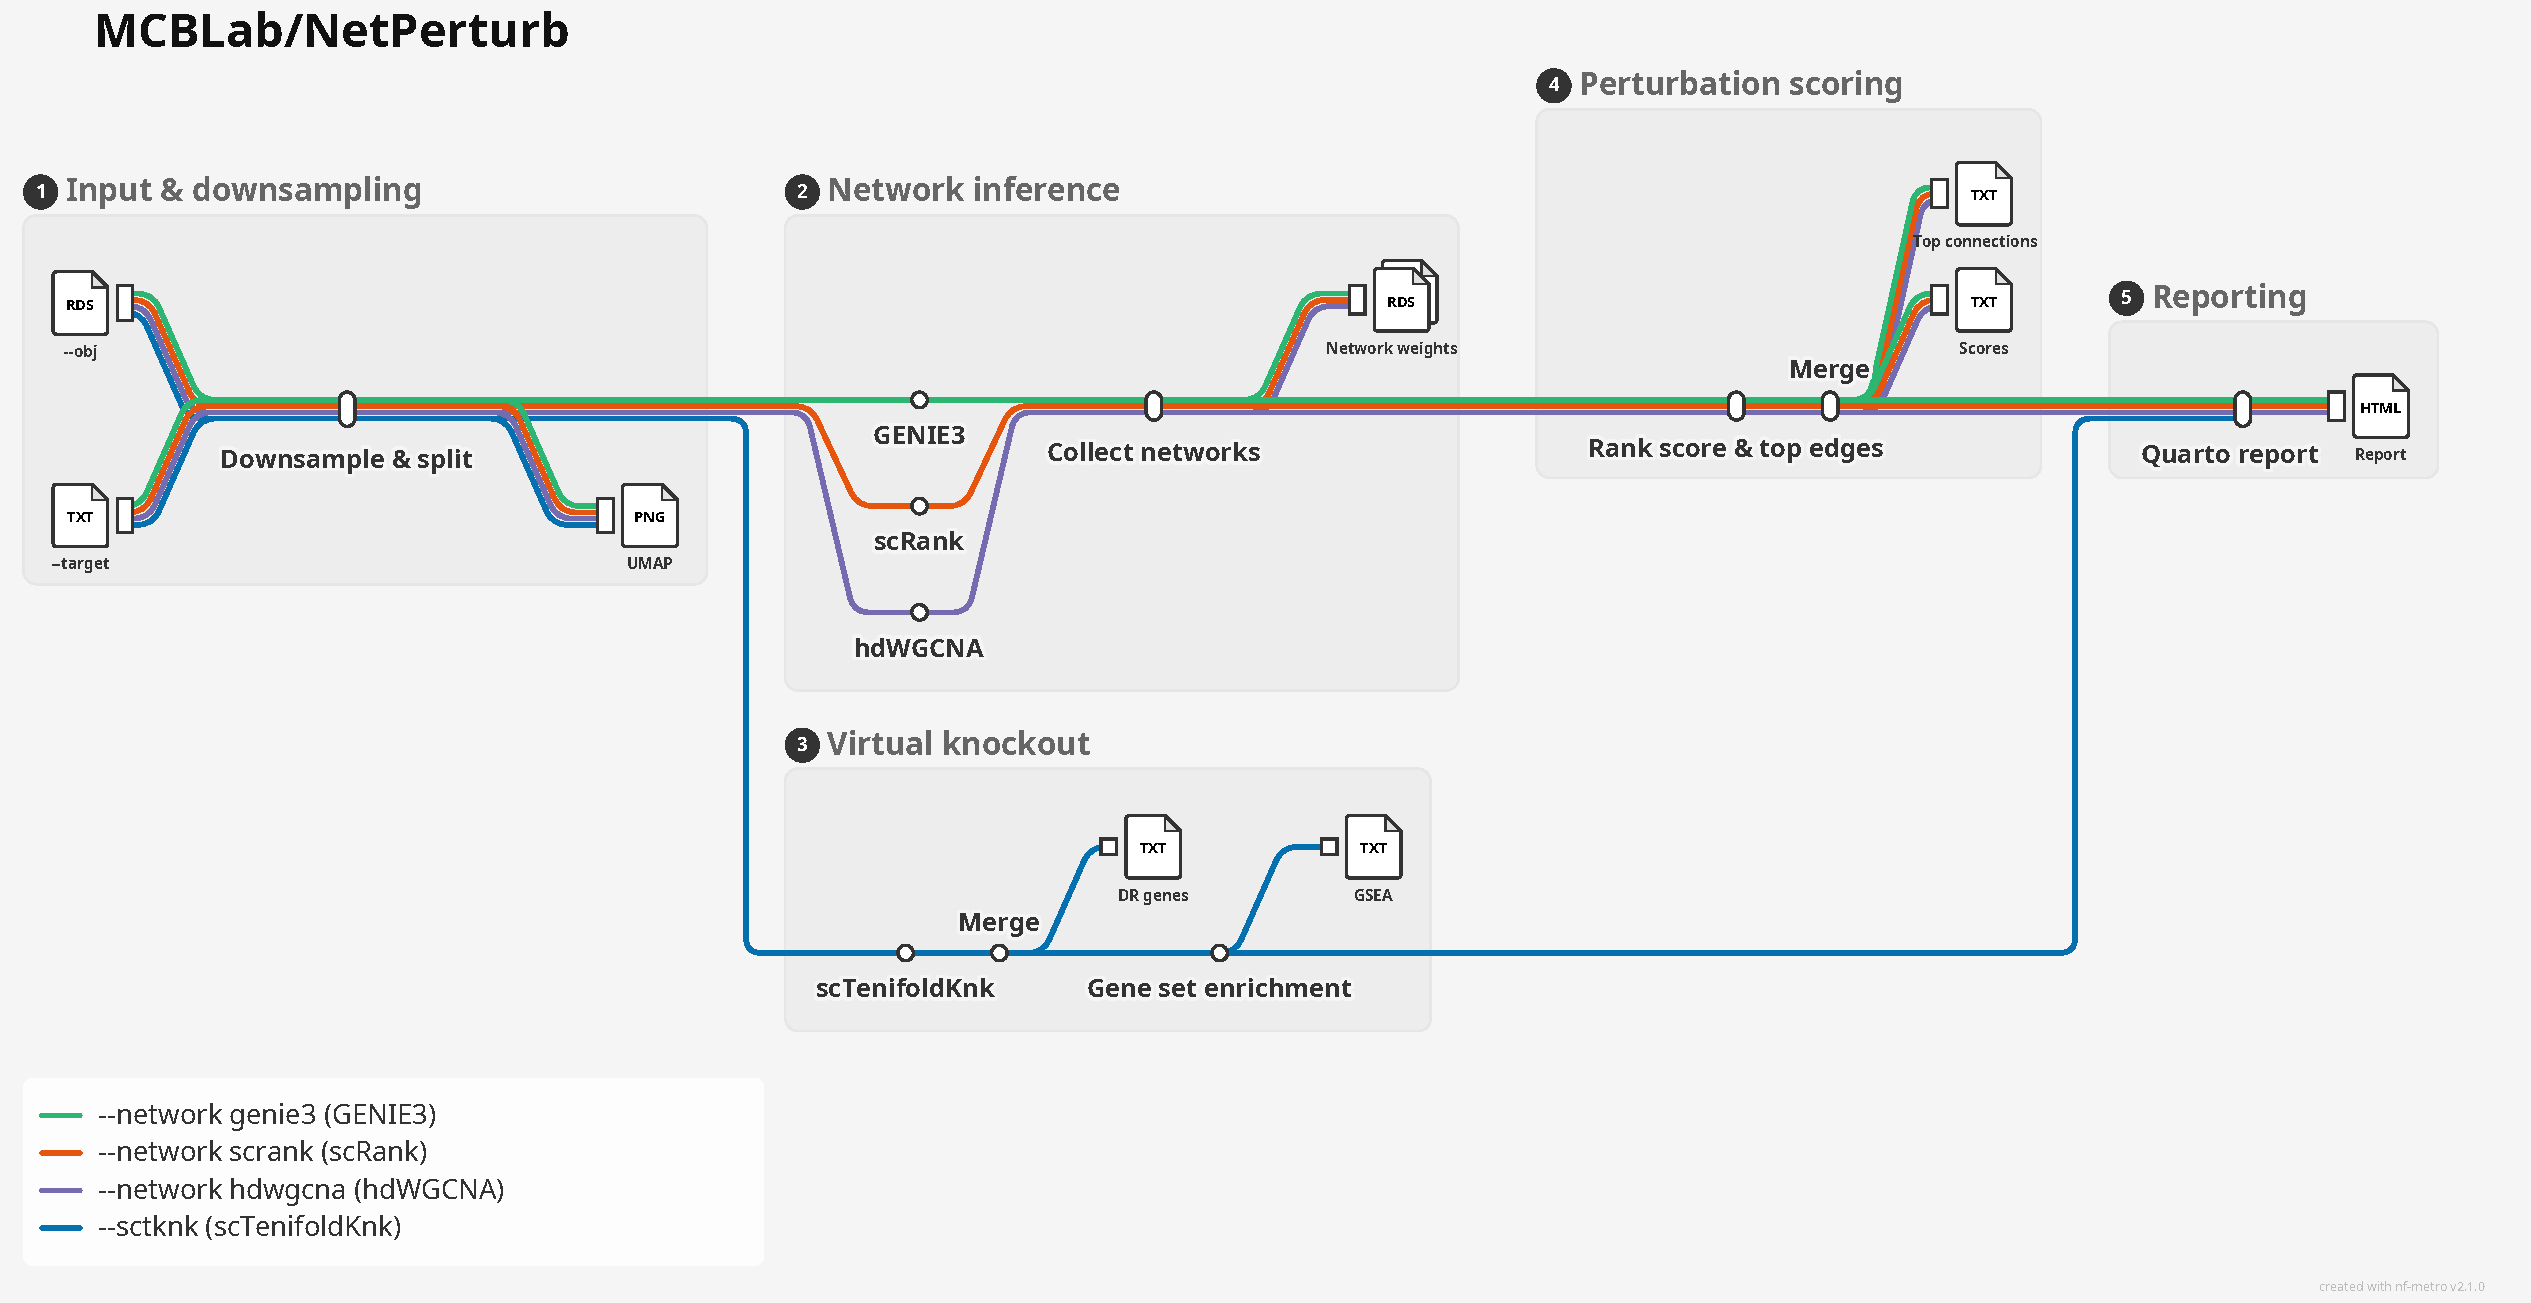
\includegraphics[width=\textwidth]{fig1_metro.pdf}
\caption{\textbf{Overview of NetPerturb.} A processed Seurat object and a list of target genes enter \texttt{DOWNSAMPLE}, which balances cell identities and checks the targets. The rank-score track (warm lines; one of GENIE3, scRank or hdWGCNA, chosen with \param{network}) infers one GRN per identity and scores every identity $\times$ target pair. The knockout track (blue; \param{sctknk}) builds one wild-type scTenifoldKnk network per identity and runs one virtual knockout per identity $\times$ target, optionally followed by fgsea. Both tracks converge on a single self-contained HTML report.}\label{fig:overview}
\figalttext[Metro-map diagram of the NetPerturb pipeline]{Metro-style diagram in which coloured lines represent the three alternative network inference methods and the parallel scTenifoldKnk knockout track, running from input through downsampling, network inference, scoring, merging and enrichment to the HTML report.}%
\end{figure*}

\subsection{Input and pre-processing}

NetPerturb requires four inputs: a Seurat object (\param{obj}), the metadata column defining cell identities (\param{column}), the species, and a text file of targets (\param{target}), one per line. Genes joined by a semicolon (e.g.\ \texttt{CDK8;CDK19}) are treated as a single combined perturbation. The \texttt{DOWNSAMPLE} step randomly keeps at most \param{n\_cells} cells per identity, so that every identity contributes a comparable number of cells, and drops identities that end up with fewer than \param{min\_cells} cells. It also builds a shared gene universe from the highly variable genes, transcription factors, drug targets and the requested targets. Each target is checked against the retained cells before any network is built. Genes that are absent from the object or have no counts are removed and recorded, a combined target keeps whichever of its genes pass, and the run stops only when no target passes. Problems that would otherwise end a run hours later are therefore caught at the start and listed in the report.

\subsection{Rank-score track}

For each identity, NetPerturb infers a GRN with one of three interchangeable methods (Table~\ref{tab:methods}). GENIE3 \citep{HuynhThu2010genie3} and scRank's own network builder \citep{Li2024scrank} are used as published. hdWGCNA \citep{Morabito2023hdwgcna}, which builds on WGCNA \citep{Langfelder2008wgcna}, produces an unsigned co-expression network on metacells, so NetPerturb adapts its topological overlap matrix to the input scRank expects in four steps. It restores the sign of each edge from the correlation between the two genes, pads every identity to the same gene set, removes edges below the \param{cut\_ratio} quantile of absolute weight, and rescales the weights to $[-1,1]$. Each identity $\times$ target pair is then scored with scRank, which compares each network before and after removing the target's edges and returns a perturbation score in either antagonist or agonist mode. The strongest \param{top\_connections} edges of each target are also exported. Networks and scores are computed as separate parallel tasks and merged into one table afterwards.

\begin{table}[!t]
\begin{center}
\begin{minipage}{\columnwidth}
\caption{Network inference methods available in NetPerturb.\label{tab:methods}}%
\small\begin{tabular}{@{}llll@{}}
\toprule
Method & Network & Output & Track \\
\midrule
GENIE3      & Tree-based regression  & Directed weights       & Rank score \\
scRank      & scRank builder   & Directed weights       & Rank score \\
hdWGCNA     & Metacell TOM + sign    & Signed, sparsified     & Rank score \\
scTenifoldKnk & PCR + tensor denoising & WT vs.\ KO manifold  & Knockout \\
\botrule
\end{tabular}
\begin{tablenotes}%
\item TOM, topological overlap matrix; PCR, principal component regression; WT, wild type; KO, knockout.
\end{tablenotes}
\end{minipage}
\end{center}
\end{table}

\subsection{Virtual knockout track}

When \param{sctknk} is set, a scTenifoldKnk track \citep{Osorio2022sctenifoldknk} runs alongside the rank-score track, or on its own. The expensive wild-type network does not depend on the target, so NetPerturb builds it once per identity (\texttt{SCTENIFOLDKNK\_BUILD}). Each identity $\times$ target knockout then runs as a separate task on that stored network (\texttt{SCTENIFOLDKNK\_KO}). With a single build per identity, one wild-type network can serve any number of knockouts, and the knockout of a combined target can zero the edges of all its genes at once, which the original single-gene interface does not allow. Differential regulation uses the statistic of scTenifoldKnk v1.0.3, which leaves the knocked-out genes out of the reference mean. \todo{Briefly justify, e.g. ``In our tests, including them inflated the mean so much that almost no gene reached significance (1 vs.\ 12 genes at FDR $<0.05$ on a 5,600-gene network).''} If a GMT file is supplied, genes are ranked by $\log_2$FC and tested with fgsea \citep{Korotkevich2016fgsea} against, for example, MSigDB collections \citep{Liberzon2015msigdb}. Gene sets are read from local files, so the step also runs on compute nodes without internet access.

\subsection{Report}

The \texttt{REPORT} step renders a single self-contained Quarto HTML file (\todo{Supplementary Fig.~S1: report screenshots}). The report contains:
(i) an overview recording the network method, the targets removed by quality control, the number of cells and genes available to each identity's network, and a UMAP of the retained cells;
(ii) a heatmap of target expression per identity, so that a low score can be checked against a target that is barely expressed;
(iii) a searchable table and a heatmap of perturbation scores;
(iv) interactive knockout networks and a table of differentially regulated genes;
(v) an enrichment dot plot and table; and
(vi) provenance, with the command line, software versions, parameters and the running time of each step taken from the Nextflow trace.

\subsection{Reproducibility and deployment}

Every tool runs in a versioned Singularity/Docker container \citep{Kurtzer2017singularity}, so no R dependencies need to be installed. A single \param{seed} parameter sets the random seed of every step that uses one: downsampling, GENIE3 (via doRNG), hdWGCNA metacells, scTenifoldKnk and fgsea. scRank's network builder is the one exception, because it sets its own seed internally. Memory and CPU requests are defined per process and can be adjusted in a configuration profile. The pipeline is tested with nf-test at the module and workflow level, and it provides small and dataset-scale test profiles (\texttt{-profile test}).

%% =====================================================================
\section{Results}
%% =====================================================================
%% Numbers below are produced by analysis/fig2_kang.R -> analysis/kang_stats.txt

We benchmarked NetPerturb on the unstimulated (control) peripheral blood mononuclear cells of \citet{Kang2017demuxlet}, scoring 25 targets in agonist mode with hdWGCNA networks and running the scTenifoldKnk track with GO gene sets (MSigDB C5). The targets fall into three groups: the type I interferon (IFN) receptor and signalling cascade (IFNAR1, IFNAR2, JAK1, TYK2, STAT1, STAT2, IRF9 and the joint targets IFNAR1;IFNAR2, JAK1;TYK2, STAT1;STAT2); ten interferon-stimulated genes (ISGs); and five lineage genes used as controls (CD19, MS4A1, IL4R, TLR4, CSF1R). With \param{n\_cells}~2,000 and \param{min\_cells}~500, six identities were kept (7,502 cells) and two were dropped automatically (dendritic cells, 258 cells; megakaryocytes, 63 cells). Every target passed QC.

\paragraph{Monocytes rank first, but partly for every target.} Monocytes had the highest score for 20 of 25 targets, including all 10 ISGs (Fig.~\ref{fig:kang}A). This agrees with circulating monocytes carrying the highest baseline ISG expression in these data and being the main IFN-responsive population in PBMCs. However, when log scores are decomposed into target and identity effects, both monocyte populations score about 7-fold higher than the other identities regardless of target (+0.84 and +0.87 $\log_{10}$ relative to B cells). This offset also lifts the lineage controls: FCGR3A$^+$ monocytes rank first for CD19. Only after the offset is removed does the ISG signal become specific. ISGs keep a monocyte excess of 0.39 $\log_{10}$ (Wilcoxon $P=0.009$), whereas the upstream cascade shows none ($-0.14$) and the lineage controls fall below it ($-0.61$) (Fig.~\ref{fig:kang}B). The networks themselves support this: 67\% of the 15 strongest partners of an ISG in monocytes are other ISGs, against 25\% in other identities and 1\% for lineage genes (Fig.~\ref{fig:kang}C). Scores correlate moderately with target expression (Spearman $\rho=0.49$), but the monocyte term remains after adjusting for expression (0.77 $\log_{10}$, $P=6\times10^{-9}$). Targets with no counts in an identity score at the numerical floor ($<10^{-10}$, 9 pairs), as expected for an isolated node. A further 12 pairs whose target is detected in fewer than 1\% of cells still received ordinary scores, and one of them (CD19 in FCGR3A$^+$ monocytes) ranked first. \todo{Validate against the stimulated half of the data: correlate per-identity scores with the number of IFN-$\beta$-induced DE genes per cell type from the stimulated vs.\ control comparison.}

\paragraph{The knockout track is largely target-independent in this run.} All 141 identity $\times$ target knockouts produced at least one differentially regulated (DR) gene at FDR $<0.05$ (1,858 in total). The hits, however, barely depended on the target. In four of six identities the DR set was identical for most targets (median pairwise Jaccard 1.0; Fig.~\ref{fig:kang}D). In CD14$^+$ monocytes all 25 knockouts returned the same two genes, FTH1 and FTL, and the full FC rankings were highly correlated across targets (median Spearman $\rho=0.74$--$0.96$). Ribosomal protein genes made up 37\% of hits, but only 3.2\% of tested genes. The GO enrichment did not recover interferon signalling: the IFN-related sets that passed FDR $<0.25$ had negative NES, mostly in B cells. We read this as the knockout signal being dominated by genes whose network position differs between the two aligned networks for reasons unrelated to the target. \todo{Diagnose before submission: compare with scTenifoldKnk()'s own statistic (v1.1) on the same networks, a random-gene knockout null, and a larger \param{sctknk\_min\_pct}; decide whether the v1.0.3 reference mean is responsible.}

\paragraph{Cost.} The whole run took 5.0\,h of compute across all tasks (Fig.~\ref{fig:kang}E). Network inference (hdWGCNA, about 1\,min per identity) and scoring (about 31\,s per target) were small next to the scTenifoldKnk wild-type build (43\,min per identity). Building that network once per identity and reusing it for each of the 150 knockouts (5.5\,s each) took 4.5\,h, whereas one \texttt{scTenifoldKnk()} call per identity $\times$ target pair would have taken an estimated 108\,h, about 24-fold more.

\begin{figure*}[!t]%
\centering
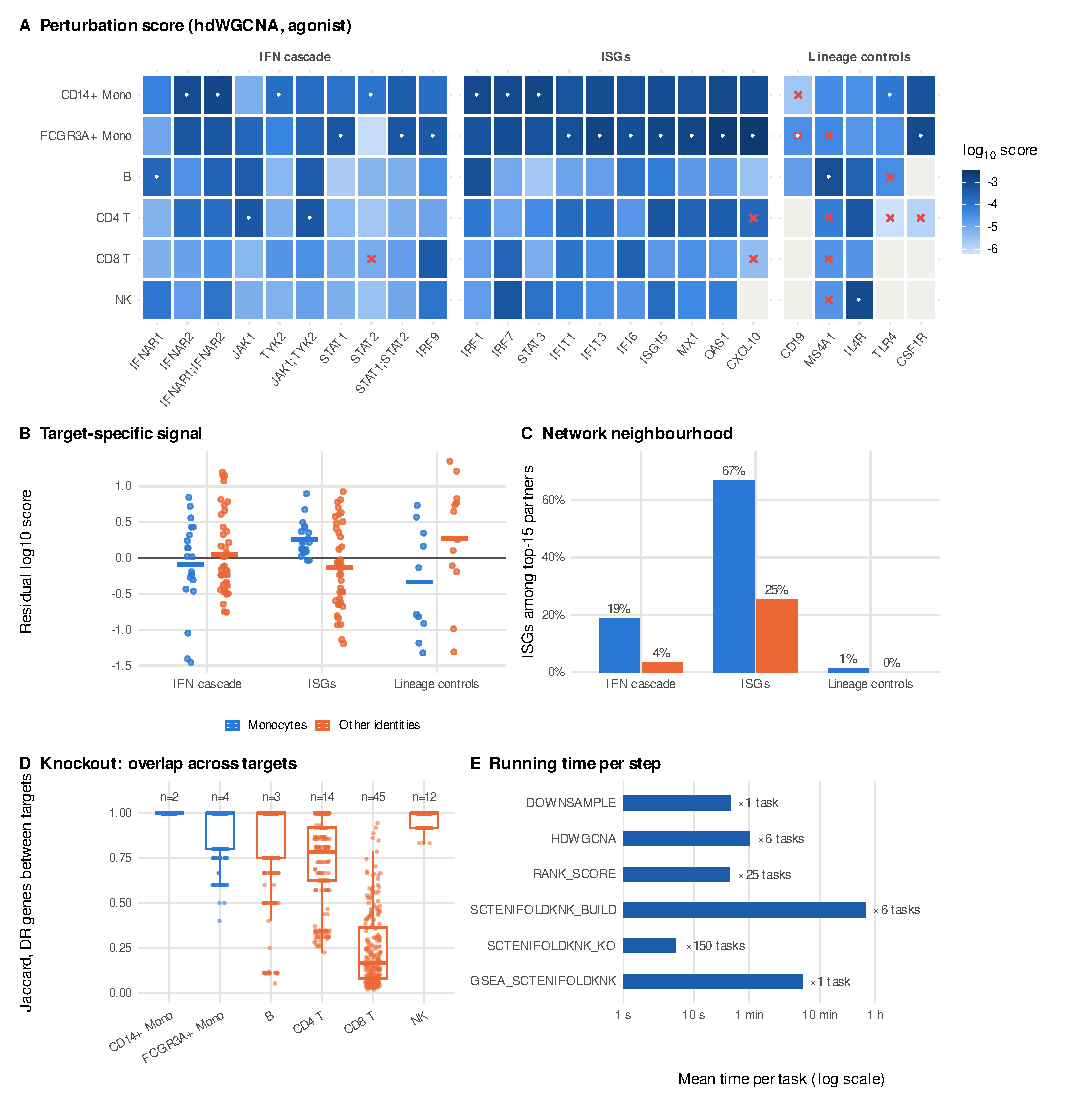
\includegraphics[width=\textwidth]{fig2_kang.pdf}
\caption{\textbf{Benchmark on unstimulated PBMCs \citep{Kang2017demuxlet}} (hdWGCNA networks, agonist mode, seed 1). (A) $\log_{10}$ perturbation score for each identity $\times$ target pair. A white dot marks the top identity for each target; a red $\times$ marks a target detected in $<1\%$ of the identity's cells; grey marks scores at the numerical floor ($<10^{-10}$). (B) Residual $\log_{10}$ score after removing the target and identity main effects, by target group; bars show means. (C) Share of each target's 15 strongest network partners (\texttt{top\_connections}) that are ISGs. (D) Pairwise Jaccard index of the scTenifoldKnk DR gene sets (FDR $<0.05$) between targets within each identity; $n$, median DR genes per target. (E) Mean running time per task for each step, from the Nextflow trace.}\label{fig:kang}
\figalttext[Five-panel benchmark figure on Kang PBMC data]{Panel A is a heatmap of perturbation scores across six cell types and 25 targets, darkest in the two monocyte rows. Panel B shows residual scores by target group, with monocytes above zero only for ISGs. Panel C is a bar chart showing that 67 percent of monocyte ISG network partners are ISGs. Panel D shows knockout gene-set overlap close to 1 in most cell types. Panel E is a bar chart of running time per pipeline step on a log scale, dominated by the scTenifoldKnk network build.}%
\end{figure*}

%% =====================================================================
\section{Conclusion}
%% =====================================================================

NetPerturb takes an analyst from a Seurat object to a shareable report on GRN-based in silico perturbation with a single command. It runs several network inference methods and a virtual knockout under one interface, and its seeding, containers and provenance make each result reproducible. The benchmark also shows how these scores should be read. Perturbation scores carry an identity-wide offset, so they should be compared against control targets from the same run rather than taken at face value; scores for targets detected in very few cells are unreliable; and knockout results that do not change with the target need a null model before they are interpreted. Scores are comparable only within one inference method, and knockout effects describe network structure, not the direction of expression change. \todo{Future work: e.g.\ built-in control targets and a per-identity null, detection filter on targets, AnnData input, nf-core submission.}

%% =====================================================================
%% Back matter -- all required by Bioinformatics Advances
%% =====================================================================

\section{Acknowledgements}
\todo{Acknowledgements.} \todo{AI disclosure: the guidelines require disclosing any AI/LLM use (e.g.\ assistance with code or drafting) here or in Methods, as well as in the cover letter.}

\section{Author contributions}
\todo{CRediT roles, e.g.\ D.M.-C.: Conceptualization, Software, Writing -- original draft. \ldots}

\section{Conflict of interest}
None declared.

\section{Funding}
\todo{Funding agencies and grant numbers.}

\section{Data availability}
The source code, container recipes and test data definitions are available at \url{https://github.com/MCBLab/NetPerturb} (release \todo{vX.Y.Z}, archived at Zenodo \todo{DOI}). The benchmark uses the data of \citet{Kang2017demuxlet} (GEO accession GSE96583); the processed Seurat object and the benchmark outputs are available at \todo{Zenodo DOI}.

%% ---------------------------------------------------------------------
%% References: numbers are capped at 15 for an Application Note.
%% references/references.bib also holds uncited entries (GEARS, van Galen, Ocasio)
%% that are not cited yet, in case you want to swap them in.
%% ---------------------------------------------------------------------
\bibliographystyle{oup-abbrvnat}
\bibliography{references/references}

\end{document}
